\renewcommand{\times}{\sffamily}

\title{AMVARA DASHBOARD}
\author{
        Amvara Consulting S.L.\\
}
\date{\today} %% Adds today date

\documentclass[11pt]{article}
\usepackage[legalpaper, margin=3cm]{geometry}
\usepackage{hyperref}
\usepackage{graphicx}
\graphicspath{ {.images/} }
\setlength{\parindent}{0pt}

%%%%%%%%%%%%%%%%%%%%%%%%%%%%%%%%%%%%%%%%%%%%%%%%%%%%%%%%%%%%%%%%
%					  	 BEGIN DOCUMENT	 					   %
%%%%%%%%%%%%%%%%%%%%%%%%%%%%%%%%%%%%%%%%%%%%%%%%%%%%%%%%%%%%%%%%


\begin{document} 
\maketitle %% Prints title and author

\begin{centering} %% Displays an image and webpage url centered
	
\includegraphics{amvara} \par
	\url{https://www.amvara.de} \par
\end{centering}

\newpage %% Page break
\tableofcontents %% Display's Table of contents
\newpage



\section{Introduction} %% First Section
This dashboard loads data from server via XHR requests and (depending on server speed) is able to visualize data in under 1 second. This documentation describes how to modify the data to fit your needs and how to change the skinning to meet your styleguide.

\subsection{Dashboard's Main Page}

The main page is divided in two parts. First we have the graphic, it is sorted by ticket type. Next, in the right part (If we are on desktop), or, in the bottom part (If we are on mobile), there are 4 tables with monthly information for each data type. It shows totals and percentages\par
\begin{center}
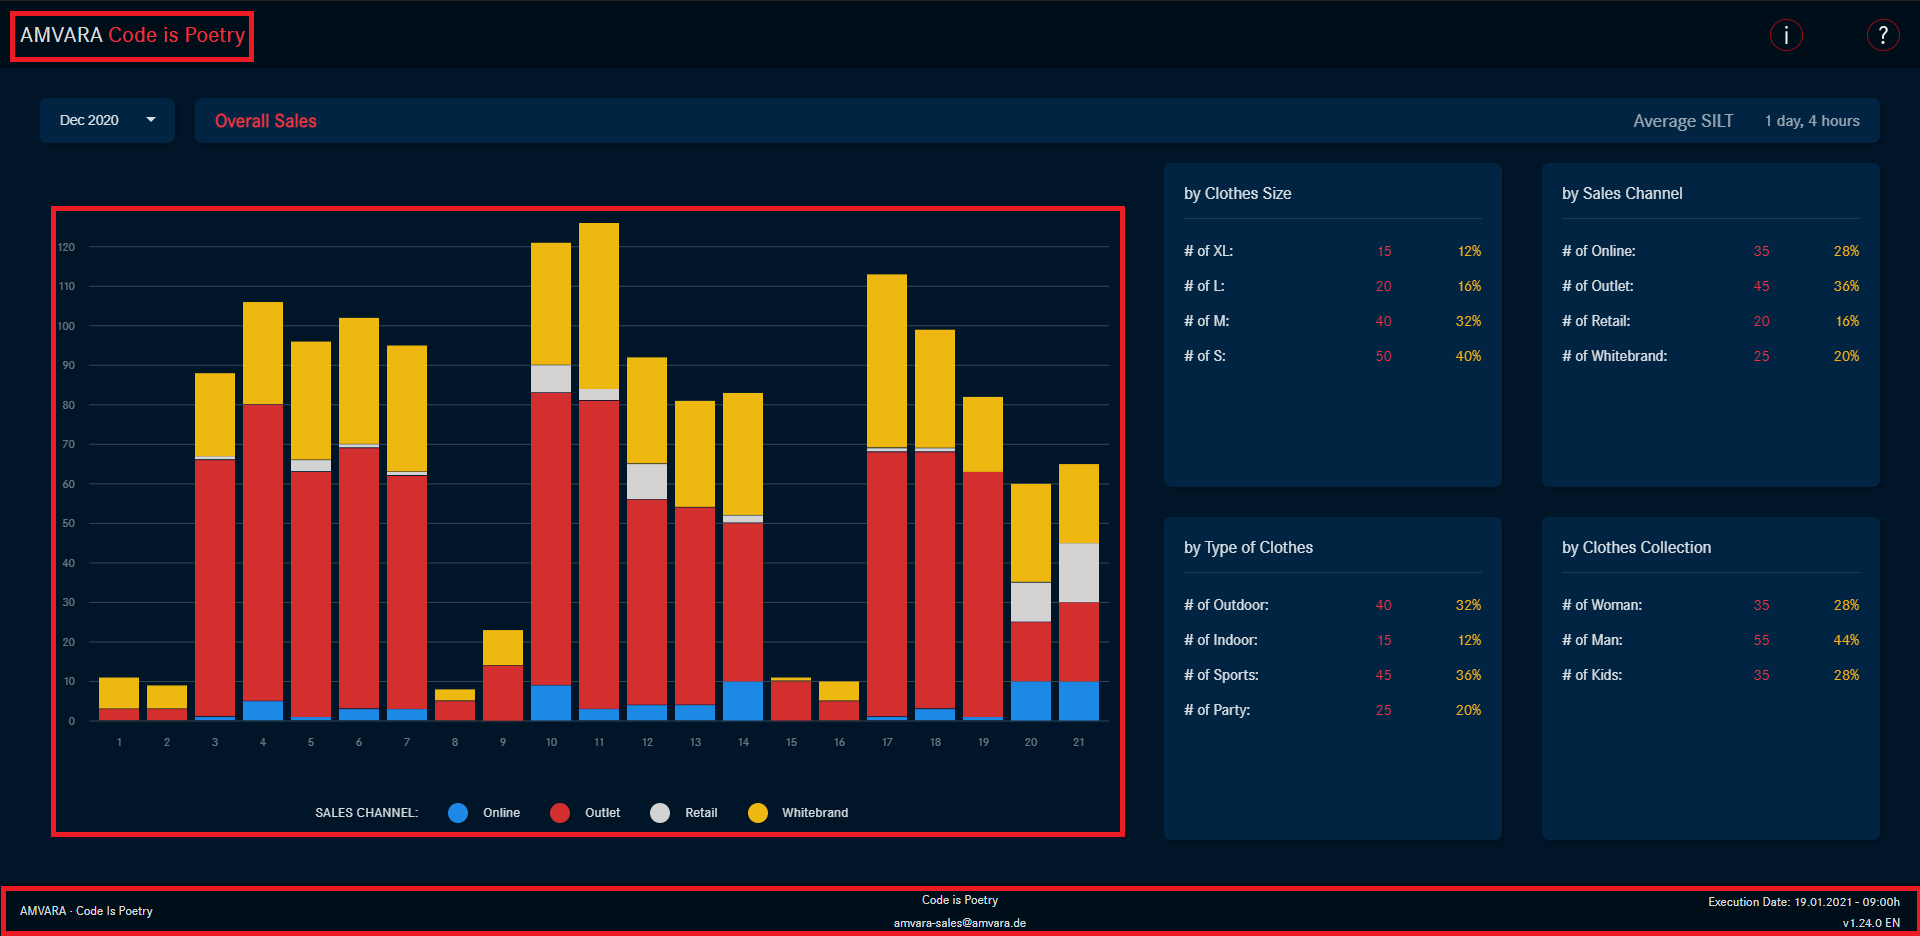
\includegraphics[
  width=440px,
  keepaspectratio,
]{principal}
\end{center}
Data can be ordered by:
\begin{itemize} %% Unordered List with dots
	\item By Priority [1,2,3,4] Being 1 the most critical and 4 the less critical
	\item By Ticket Type
	\item By Application/Service
	\item By Status
\end{itemize}
\textbf{Note:} All of these can be changed, for example. Instead of Ticket Type, Sales Channel, instead of By priority, by Clothes Size, etc. Everything can be modified according to your needs.\par
\newpage %% Page break

%%%%%%%%%%%%%%%%%%%%%%%%%%%%%%%%%%%%%%%%%%%%%%%%%%%%%%%%%%%%%%%%
%					Prepare Skinning Section				   %
%%%%%%%%%%%%%%%%%%%%%%%%%%%%%%%%%%%%%%%%%%%%%%%%%%%%%%%%%%%%%%%%
\newpage
\section{Prepare Skinning} %% Second Section
In this section, we will see how to change the dashboard skinning to meet your styleguide.

\subsection{Header}
Header title, is edited in .src/app/components/ux/header/header.component.html.The original title is ``AMVARA Code Is Poetry'', in order to change the title we will edit both span:\par
\begin{center} %% Image Centered
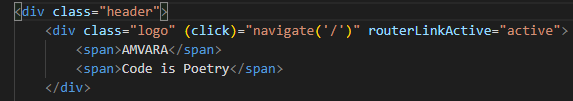
\includegraphics[
  width=300px,
  keepaspectratio,
]{header}
\end{center}
First span is shown in white color, the second one, in red. (How to change colors is explained later).

\subsection{Window Title}
Window title is edited on ./src/index.html. In order to edit it, simply change ``AMVARA DASHBOARD'' inside the title tag, with, ``YOUR DASHBOARD TITLE''.\par
\begin{center} %% Image Centered
	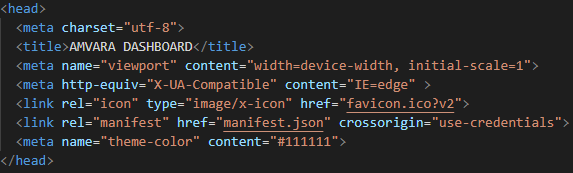
\includegraphics[
	width=300px,
	keepaspectratio,
	]{title}
	\end{center}

\subsection{Loading Screen}
Loading screen is edited on ./src/index.html
\subsubsection{Loading Screen Title}
In order to change the title, div class name must be edited. The part inside ``b'' tag will be displayed with the color specified in ``blue'' class.\par
\begin{center} %% Image Centered
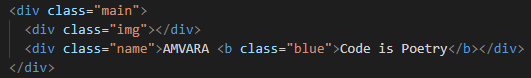
\includegraphics[
	width=300px,
	keepaspectratio,
  ]{loader}
  \end{center}
\subsubsection{Loading Screen CSS}
In order to change the ``blue'' class color, simply, find inside index.html style the blue selector and change the color to your needs:
\begin{center} %% Image Centered
	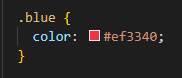
\includegraphics[
		width=90px,
		keepaspectratio,
	  ]{blue}
	  \end{center}
\pagebreak
In order to change the progress bar color, you have to edit ``.progress .progress-value'' inside index.html styles. If you want the bar to have a different background, change background-color inside .progress. If the color in .progress is the same as the background color of the dashboard, the bar will not have a visible background\par
\begin{center} %% Image Centered
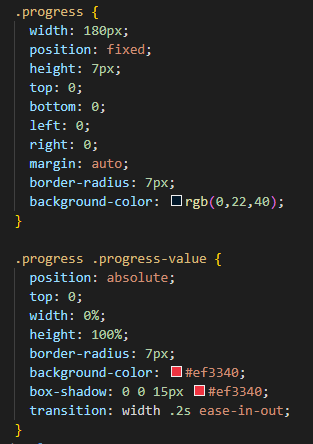
\includegraphics[
	height=200px,
	keepaspectratio,
  ]{loader-css}
  \end{center}
If you want to change the background color, edit the background-color property in the body style selector.\par
\begin{center} %% Image Centered
	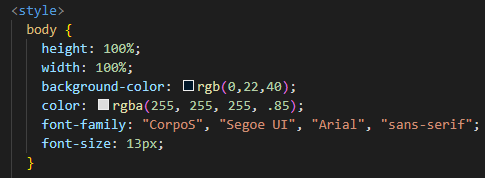
\includegraphics[
		width=200px,
		keepaspectratio,
	  ]{loaderbg}
	  \end{center}
For changing the color of the first part of the title, edit the color property in the name class style selector.
\begin{center} %% Image Centered
	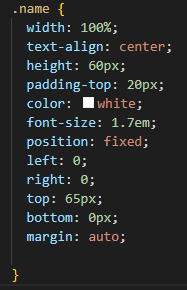
\includegraphics[
		height=200px,
		keepaspectratio,
	  ]{loadercolor}
	  \end{center}
\newpage

\subsection{General Information}
General information is edited in ./src/assets/config.json. We will have to edit the contact part:\par
\begin{center} %% Image Centered
	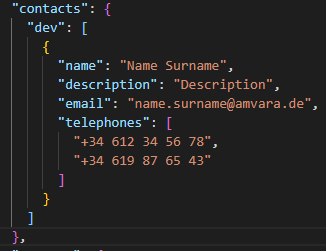
\includegraphics[
		width=200px,
		keepaspectratio,
	  ]{contact}
\end{center}

\textbf{NOTE:} Description can have more than one line.\par
\smallskip
\textbf{NOTE:} If more telephones are needed, just add a comma behind the last one and add another number.\par
\subsection{Footer}
Left footer text, is composed by copyright and appTitle, located in the config.json.\par
\begin{center} %% Image Centered
	\includegraphics[
		height=200px,
		keepaspectratio,
	  ]{appTitle}
\end{center}
Mid and right footer text, are edited in .src/app/components/ux/footer/footer.component.html:\par
\begin{center} %% Image Centered
	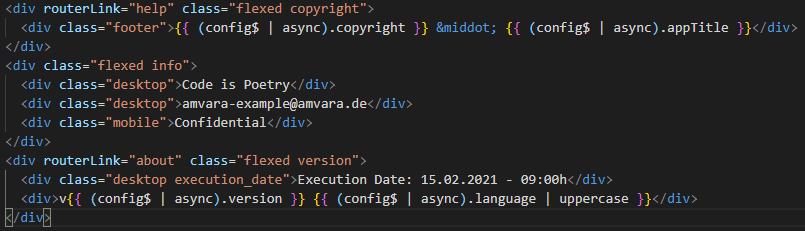
\includegraphics[
		width=400px,
		keepaspectratio,
	  ]{footer-info}
\end{center}
Inside div class flexed, is located the middle text, the text shown will depend if it is accesed from a desktop or a mobile. Then we have the flexed version, that display the execution date and the version of the dashboard.\par
\newpage
\subsection{Colors}
Dasboard's colors, are edited in ./src/app/common/\_colors.scss.\par
\begin{center} %% Image Centered
	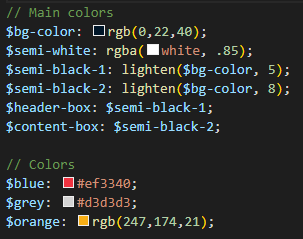
\includegraphics[
	height=150px,
	keepaspectratio,
	]{colors}
\end{center}
The color variables to edit in order to change dashboard colors are:\par
\begin{itemize} %% Unordered List with dots
	\item \$bg-color: Dashboard's background color.
	\item \$semi-white: Dashboard's text color.
	\item \$blue: Dashboard's colors for title and total numbers.
	\item \$grey: General information telephone color.
	\item \$orange: Will change percentage text color and general information link.
\end{itemize}

\subsection{Chart Legend and colors}
In order to change chart legend and colors, the file config.json must be edited. it is located in ./src/assets/config.json\par
\begin{center} %% Image Centered
	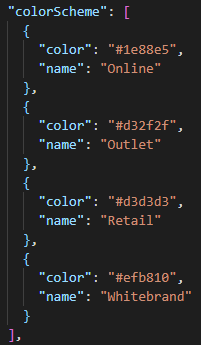
\includegraphics[
	height=250px,
	keepaspectratio,
	]{colorscheme}
\end{center}
Colors are changed in ``color'' and legend names are changed in ``name''\par

%%%%%%%%%%%%%%%%%%%%%%%%%%%%%%%%%%%%%%%%%%%%%%%%%%%%%%%%%%%%%%%%
%				   Introducing Data Section					   %
%%%%%%%%%%%%%%%%%%%%%%%%%%%%%%%%%%%%%%%%%%%%%%%%%%%%%%%%%%%%%%%%
\newpage
\section{Introducing Data} %% Section three \_ \_ of filename.csv needed to print _
The data insertion or edition is done by editing the file Mobile\_List\_Chart.csv (Located in .src/assets/reports/), it is mandatory to use the same name in the ticket type column  inside the csv and in the colorscheme inside config.json (Located in .src/assets/). If not, when clicking in the bar chart, data will not be displayed correctly.\par

\subsection{dashboardhelper.sh}
Every time Mobile\_List\_Chart.csv is modified, it is important to execute dashboardhelper.sh (Located in .scripts/), this script will read the csv and will complete the other CSV files such as Mobile\_Tickets\_Priority.csv or Mobile\_Tickets\_Service.csv, among others. it is very simple to run the script, just open a terminal in ./scripts folder and run ./dashboardhelper.sh -m. For futher information, run ./dashboardhelper -h or ./dashboardhelper --help\par

\subsection{Table Column Names}
In order to change column names to your needs, edit ``cell\_header'' in the language files inside src/assets/i18n.\par
\begin{center} %% Image Centered
	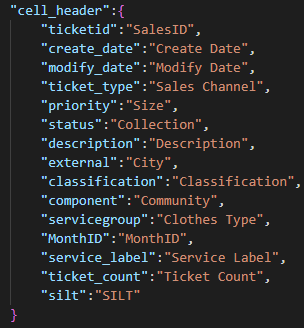
\includegraphics[
	height=220px,
	keepaspectratio,
	]{columns}
\end{center}

%%%%%%%%%%%%%%%%%%%%%%%%%%%%%%%%%%%%%%%%%%%%%%%%%%%%%%%%%%%%%%%%
%				    Configure XHR Section					   %
%%%%%%%%%%%%%%%%%%%%%%%%%%%%%%%%%%%%%%%%%%%%%%%%%%%%%%%%%%%%%%%%
\section{Configure XHR}
In order to configure XHR, ``fullUrl'' and ``portalFolder'' must be edited inside config.json. In \textbf{fullUrl} you have to specify the protocol and domain, for example:\\\textbf{``https://www.yourdomain.com''}. In \textbf{portalFolder} you have to specify the route to the main page, for example: \textbf{``/your/route''}, this URL's will be concatenated so the final url wil be \textbf{``https://www.yourdomain.com/your/route''}.\par
\bigskip

\textbf{Note:} portalFolder can be empty if main page is located in \textbf{``/''}.\par
\smallskip

\textbf{Note:} It is important to be careful with ``/'' in fullUrl and portalFolder, for example, if fullUrl is \textbf{``https://www.yourdomain.com/''} and portalFolder is \textbf{``/your/route''} your final URL will be \textbf{``https://www.yourdomain.com//your/route''}. So you can specify it at the end of fullUrl or at the start of portalFolder, but not in both of them.	\par

\subsection{Configure IBM Cognos}

\end{document} %% End of document
